\section{粒子群}
\label{sec:rs-pso}

演化策略让分布移动，遗传算法重组编码。还有一种组织方式：让每个候选都带着速度在连续空间中移动，并记住自己和同伴到过的好位置。这称为\term{粒子群优化}（particle swarm optimization，PSO）。接下来要弄清：怎样利用已发现的位置引导移动，移动的幅度由什么控制？

可以把它想成一群人在雾中找谷底，每人记得自己到过的最低处，也听得到一些同伴报告的最低处。每一步他沿惯性继续走，同时被这两个记忆的方向拉一下。这个比喻只对应更新公式的结构，不能推出任何收敛性质。

\subsection{个人与群体记忆}
\label{sec:rs-pso-memory}

粒子的移动依赖记忆。这一小节的问题是：每个粒子要记住什么，同伴之间共享什么？

\paragraph{完整状态}
设有$N$个粒子，变量是$\bm{x}\in\mathbb{R}^n$。第$i$个粒子第$t$步的状态由四个量组成：
\begin{itemize}
 \item 位置$\bm{x}_i^{(t)}$：当前候选；
 \item 速度$\bm{v}_i^{(t)}$：上一步的位移，不是目标的导数；
 \item \term{个人最好位置}（personal best）$\bm{p}_i^{(t)}$：这个粒子到过的最好位置；
 \item \term{邻域最好位置}（neighborhood best）$\bm{g}_i^{(t)}$：指定邻域内各粒子的个人最好位置中最好的一个。
\end{itemize}
本节的$\bm{g}_i$是位置，不是梯度。

初始化时在搜索区域内均匀抽位置，抽较小的初速度，评价一遍，令$\bm{p}_i^{(0)}=\bm{x}_i^{(0)}$，然后由定义得到$\bm{g}_i^{(0)}$。

个人记忆的更新规则是：
\begin{equation}
 \bm{p}_i^{(t+1)}=
 \begin{cases}
  \bm{x}_i^{(t+1)},&f(\bm{x}_i^{(t+1)})<f(\bm{p}_i^{(t)}),\\
  \bm{p}_i^{(t)},&\text{否则}.
 \end{cases}
 \label{eq:rs-pso-pbest}
\end{equation}
相同评价值时规定不更新，这样结果不依赖浮点上的偶然差别。在邻域内比较时，若有并列，按粒子编号取最小者，也要事先固定。

\paragraph{共享范围}
图~\ref{fig:rs-pso-topology}是两种共享方式。\textbf{全局共享}时所有粒子彼此相连，$\bm{g}_i$对所有$i$相同，就是全体个人记忆中最好的一个。\textbf{局部邻域}时每个粒子只与环上的相邻粒子交换信息，好位置要经过多步才能传遍全群。

\begin{BookInlineFigure}
 \centering
 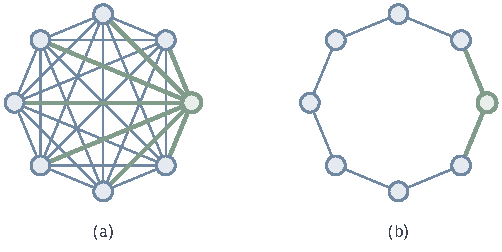
\includegraphics[width=85mm]{figures/05-optimization/05-stochastic-optimization/tikz/rs-pso-topology/figure.pdf}
 \caption{八个粒子的两种信息共享方式，绿色圆是当前关注的粒子，绿线是它能直接获知的同伴。(a)全局共享：每个粒子能看到其他所有粒子。(b)环形邻域：只与左右两个粒子交换。}
 \label{fig:rs-pso-topology}
\end{BookInlineFigure}

全局共享传播快，全群容易一起挤向同一个地方；环形邻域传播慢，不同区段可以暂时朝不同的好位置移动，保留较多的探索。

\paragraph{同步与异步}
实现上有两种顺序。\textbf{同步}更新时，一轮内所有粒子都用上一轮结束时的记忆移动，全部评价完再统一更新记忆，这便于并行评价。\textbf{异步}更新时，每评价完一个粒子，立即更新记忆，后面的粒子马上能用到新发现。两者的结果不同，记录算法时要写清楚用的是哪一种。下面用同步。

\subsection{速度与位置更新}
\label{sec:rs-pso-update}

有了状态和记忆，这一小节写出一步更新的公式，并按实际的次序算一遍。

\paragraph{主要思想}
新速度由三部分叠加：沿旧速度的惯性，朝个人记忆的拉力，朝邻域记忆的拉力。两个拉力的强度带随机性，以避免所有粒子沿同一条确定的轨迹运动：
\begin{equation}
 \begin{aligned}
 \bm{v}_i^{(t+1)}&=\bm{v}_i^{(t)}+c_1\bm{r}_{1}\odot\bigl(\bm{p}_i^{(t)}-\bm{x}_i^{(t)}\bigr)+c_2\bm{r}_{2}\odot\bigl(\bm{g}_i^{(t)}-\bm{x}_i^{(t)}\bigr),\\
 \bm{x}_i^{(t+1)}&=\bm{x}_i^{(t)}+\bm{v}_i^{(t+1)},
 \end{aligned}
 \label{eq:rs-pso-update}
\end{equation}
其中$c_1,c_2>0$是吸引系数，$\odot$表示按分量相乘，$\bm{r}_1,\bm{r}_2$的各个分量独立地均匀取自$[0,1]$，并且对每个粒子、每一轮重新抽取。

这里的差$\bm{p}_i-\bm{x}_i$和$\bm{g}_i-\bm{x}_i$只是到记忆位置的位移，不是目标的梯度。在下面的例子里$\bm{x}=(4,2)$，负梯度是$(-4,-18)$，朝邻域记忆的位移是$(-3,-1)$，两者的夹角约为$59^\circ$。粒子可以朝一个代价更高的方向飞，因为记忆里的点在那边。

\paragraph{变量}
一个粒子需要$\bm{x}$、$\bm{v}$、$\bm{p}$、$\bm{g}$，以及$f(\bm{p})$；全局还要保存历史最好记录。

\paragraph{初始化}
下面用$f(\bm{x})=\tfrac12(x_1^2+9x_2^2)$核对一步。设系数$c_1=c_2=1.5$，粒子当前状态是
\[
 \bm{x}=\begin{bmatrix}4\\2\end{bmatrix},\quad\bm{v}=\begin{bmatrix}-1\\0.5\end{bmatrix},\quad\bm{p}=\begin{bmatrix}3\\1\end{bmatrix},\quad\bm{g}=\begin{bmatrix}1\\1\end{bmatrix}.
\]
记忆处的代价是$f(\bm{p})=9$，$f(\bm{g})=5$。

\paragraph{每轮更新}
每一轮按下面的次序处理每个粒子，用完预算为止。

\begin{enumerate}
 \item 抽随机向量。例中
 \[
  \bm{r}_1=\begin{bmatrix}0.5\\0.2\end{bmatrix},\qquad\bm{r}_2=\begin{bmatrix}0.4\\0.6\end{bmatrix}.
 \]
 \item 由式~\eqref{eq:rs-pso-update}计算新速度。例中个人项和群体项分别是
 \[
  1.5\,\bm{r}_1\odot(\bm{p}-\bm{x})=\begin{bmatrix}-0.75\\-0.3\end{bmatrix},\qquad
  1.5\,\bm{r}_2\odot(\bm{g}-\bm{x})=\begin{bmatrix}-1.8\\-0.9\end{bmatrix},
 \]
 加上旧速度得到
 \[
  \bm{v}^{+}=\begin{bmatrix}-3.55\\-0.7\end{bmatrix}.
 \]
 \item 计算新位置并评价。例中
 \[
  \bm{x}^{+}=\begin{bmatrix}0.45\\1.3\end{bmatrix},\qquad f(\bm{x}^{+})=\tfrac12(0.2025+15.21)\approx7.71.
 \]
 \item 完成评价后更新记忆。例中$7.71<9$，个人记忆更新为$(0.45,1.3)$；$7.71>5$，邻域记忆$\bm{g}$不变。
\end{enumerate}

图~\ref{fig:rs-pso-vector}把这一步的三段位移画成首尾相接的箭头。这个粒子一步就把代价从$26$降到了约$7.71$，主要靠群体项。

\begin{BookInlineFigure}
 \centering
 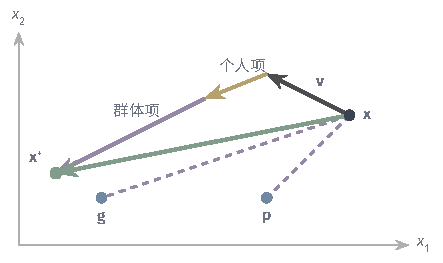
\includegraphics[width=75mm]{figures/05-optimization/05-stochastic-optimization/tikz/rs-pso-vector/figure.pdf}
 \caption{粒子的一步更新。深灰箭头是旧速度，黄箭头是个人项，紫箭头是群体项，绿箭头是合成的实际位移，虚线连向两个记忆位置。两个拉力分量的比例来自随机向量，所以合成位移不必指向任何一个记忆位置。}
 \label{fig:rs-pso-vector}
\end{BookInlineFigure}

\paragraph{速度限幅的计算}
实际常把速度各分量限制在$[-v_{\max},v_{\max}]$内。此时必须用修正后的速度计算位移。例中取$v_{\max}=2$，$\bm{v}^{+}$被截断为$(-2,-0.7)$，新位置是$(2,1.3)$，代价约为$9.61$。这比$f(\bm{p})=9$大，这一步个人记忆就不更新了。

记录下来的$\bm{v}^{+}$必须是截断后的那个，否则下一轮的惯性项与实际位移不一致。

图~\ref{fig:rs-pso-swarm}是二维Rastrigin函数上$24$个粒子的一次运行，三幅分别是第$0,8,60$轮的位置。第$8$轮粒子已聚向原点附近，第$60$轮已基本聚集，这次最好代价约为$2\times10^{-5}$。

\begin{BookInlineFigure}
 \centering
 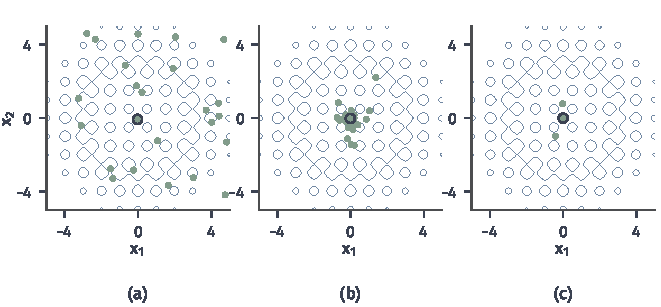
\includegraphics[width=112mm]{figures/05-optimization/05-stochastic-optimization/matplotlib/rs-pso-swarm/figure.pdf}
 \caption{二维Rastrigin函数上的粒子群，$N=24$，全局共享，带惯性权重$\omega=0.7298$，$c_1=c_2=1.496$，$v_{\max}=2$，同步更新，种子固定。(a)(b)(c)分别是第$0,8,60$轮的粒子位置（绿点），蓝线是等高线$f=30$，深色圆圈是当前的全局最好记忆，红点是全局最小点。}
 \label{fig:rs-pso-swarm}
\end{BookInlineFigure}

\subsection{移动尺度与停滞}
\label{sec:rs-pso-scale}

式~\eqref{eq:rs-pso-update}没有任何东西让速度变小。这一小节的问题是：什么控制粒子的移动尺度，粒子群停止移动时又说明了什么？

\paragraph{为什么要给速度加阻尼}
把问题简化。只看一维，记忆固定在$p=g=0$，把随机量换成常数，记$\varphi=c_1r_1+c_2r_2$。在旧速度前面乘上一个系数$\omega$（称为惯性权重），更新变成
\begin{equation}
 v^{+}=\omega v-\varphi x,\qquad x^{+}=x+v^{+}.
 \label{eq:rs-pso-deterministic}
\end{equation}
式~\eqref{eq:rs-pso-update}对应$\omega=1$。

\begin{theorem}[确定性粒子的稳定条件]
\label{thm:rs-pso-stability}
递推~\eqref{eq:rs-pso-deterministic}对任意初值都有$x^{(t)}\to0$，$v^{(t)}\to0$，当且仅当
\begin{equation}
 \lvert\omega\rvert<1,\qquad0<\varphi<2+2\omega.
 \label{eq:rs-pso-stable}
\end{equation}
\end{theorem}

\begin{proof}
把$v^{+}$代入第二式，$x^{+}=(1-\varphi)x+\omega v$，于是
\[
 \begin{bmatrix}x^{+}\\v^{+}\end{bmatrix}=\bm{M}\begin{bmatrix}x\\v\end{bmatrix},\qquad
 \bm{M}=\begin{bmatrix}1-\varphi&\omega\\-\varphi&\omega\end{bmatrix}.
\]
线性递推对任意初值收敛到零，当且仅当$\bm{M}$的两个特征值模都小于$1$。

$\bm{M}$的迹是$1-\varphi+\omega$，行列式是$\omega(1-\varphi)+\omega\varphi=\omega$，特征多项式为
\[
 \chi(z)=z^2-(1-\varphi+\omega)z+\omega.
\]

先计算两个端点的值：
\[
 \chi(1)=\varphi,\qquad\chi(-1)=2+2\omega-\varphi.
\]

两根为实数时，两根都在$(-1,1)$内，当且仅当$\chi(1)>0$，$\chi(-1)>0$，且两根之积的绝对值小于$1$，这三条合起来正是式~\eqref{eq:rs-pso-stable}。

两根为共轭复数时，$\omega>0$，模的平方等于乘积$\omega$，所以模小于$1$当且仅当$\omega<1$。此时判别式为负，给出
\[
 \lvert1-\varphi+\omega\rvert<2\sqrt{\omega}\leq1+\omega,
\]
这就是$0<\varphi<2+2\omega$，所以它自动成立。两种情形合起来，即得结论。
\end{proof}

$\omega=1$时行列式为$1$，两个特征值的模乘积为$1$，不可能都小于$1$，所以原始的式~\eqref{eq:rs-pso-update}没有衰减。图~\ref{fig:rs-pso-stability}(a)中$\omega=1$，$\varphi=1.5$的轨迹一直等幅振荡；$\omega=0.7$时振荡衰减，$45$步后已接近零。

这是把随机量换成常数后的结论，真实的$\varphi$每轮变化，乘积的稳定性与平均值的稳定性并不相同，定理只用来解释阻尼的作用。它说明了实践中必须做一件事：要么加$v_{\max}$，要么取$\omega<1$，否则粒子会越飞越散。

\begin{BookInlineFigure}
 \centering
 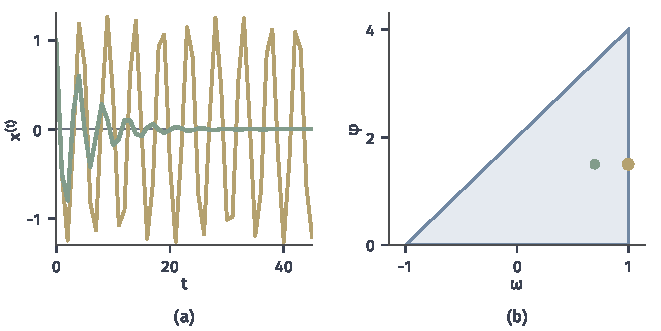
\includegraphics[width=112mm]{figures/05-optimization/05-stochastic-optimization/matplotlib/rs-pso-stability/figure.pdf}
 \caption{确定性粒子~\eqref{eq:rs-pso-deterministic}，记忆在原点，$x^{(0)}=1$，$v^{(0)}=0$。(a)$\varphi=1.5$，黄线$\omega=1$，绿线$\omega=0.7$。(b)蓝色三角形是稳定区域~\eqref{eq:rs-pso-stable}，两个点对应(a)中的两组参数，黄点位于边界上。}
 \label{fig:rs-pso-stability}
\end{BookInlineFigure}

\paragraph{三个控制量}
表~\ref{tab:rs-pso-controls}比较影响移动尺度和信息传播的三个量。它们的合适取值依赖问题和预算。

\begin{BookInlineTable}
 \centering
 \caption{粒子群的三个控制量。}
 \label{tab:rs-pso-controls}
 \begin{tabular}{lll}
  \toprule
  控制量 & 增大时 & 过度时 \\
  \midrule
  $v_{\max}$ & 允许跳得更远 & 粒子飞出搜索区域 \\
  $c_1,c_2$ & 向记忆靠拢更用力 & 振荡，越过记忆点 \\
  邻域大小 & 信息传播更快 & 全群过早聚到一处 \\
  \bottomrule
 \end{tabular}
\end{BookInlineTable}

\paragraph{越界的处理}
粒子飞出搜索区域$[\ell_j,u_j]$时，位置和速度都要处理。常用的做法是把位置截断到边界并把该分量速度置零，或者把位置反射回来并反转速度分量。

只截断位置、保留原速度是不行的：下一步粒子会继续往外冲，每一轮都贴在边界上。不管用哪一种，都要保证下一轮的$\bm{v}$与实际位移一致，这一点和速度限幅相同。第~\ref{sec:rs-constraints}节会说明，这些处理也改变了搜索的分布。

\paragraph{停滞}
考虑这样的状态：全体粒子都位于同一点$\bm{x}^\circ$，$\bm{p}_i=\bm{g}_i=\bm{x}^\circ$，$\bm{v}_i=\bm{0}$。代入式~\eqref{eq:rs-pso-update}，两个差都是零，旧速度也是零，于是不论$\bm{r}_1,\bm{r}_2$取什么值，
\[
 \bm{v}_i^{+}=\bm{0},\qquad\bm{x}_i^{+}=\bm{x}^\circ.
\]
算法从此不再移动。

这个$\bm{x}^\circ$可以是任何点。比如在$f=\tfrac12(x_1^2+9x_2^2)$上，$\bm{x}^\circ=(1,1)$的梯度是$(1,9)$，它连驻点都不是。所以粒子聚在一起、速度趋于零或者记录长期不变，都只是搜索过程的描述，不是最优性的证明。

实际运行中粒子不一定精确聚在一点，但速度变小后移动的尺度已不足以发现更好的位置，效果相同。常用的补救是重新分散一部分粒子，同时保留历史最好记录。
